\section{MIP on arbitrary polygonal cells} \label{sec_mip}
In this section, we introduce the PieceWise Linear Discontinuous (PWLD) finite
elements developed in \cite{pwld_2d,pwld_3d,pwl_diffusion}. To obtain PWLD
basis functions for two-dimensional polygons, we first divide each polygonal
cell into ``side'' sub-cells. A ``side'' sub-cell is a triangle made from two
adjacent vertices and the within-cell point $c$. The coordinates of $c$ are weighted
averages of the vertex coordinates:
\begin{align}
& x_c = \sum_{j=1}^{V} \alpha_{j} x_j\\
& y_c = \sum_{j=1}^{V} \alpha_{j} y_j
\end{align}
where $\sum_{j=1}^{V} \alpha_{j}=1$ and $V$ is the number of vertices of the cell.\\
The basis function at vertex $j$ is defined as \cite{pwld_2d}:
\begin{equation}
b_{j} (x,y) = t_{j}(x,y) + \alpha_j t_c(x,y)
\end{equation}
where the $t_j$ functions are standard linear functions on triangles: $t_j
(x,y)$ is unity at vertex $j$, zero at $j-1$, $j+1$ and $c$, and zero in all
triangular sides that are not in contact with vertex $j$. The function $t_c
(x,y)$ is unity at $c$ and zero at each vertex. The parameters $\alpha_{j}$
are arbitrary positive weights. In this paper, we use 
$\alpha_{j}=\frac{1}{V}$. On a square cell with $\alpha_{j}=0.25\ \forall j$, 
the basis functions are given in Figure (\ref{pwld}):
\begin{figure}[H]
\centering
\subfloat[First basis function]{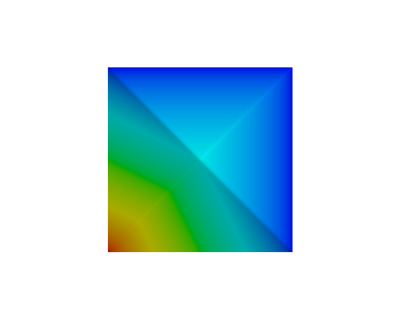
\includegraphics[width=0.3\textwidth]{pwld_1}}
\subfloat[Second basis function]{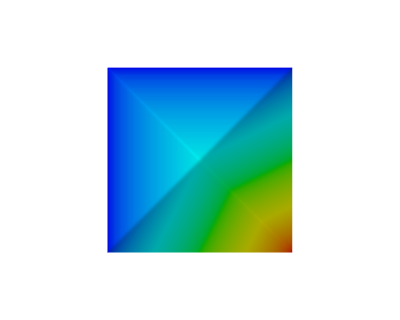
\includegraphics[width=0.3\textwidth]{pwld_2}}\\
\subfloat[Third basis function]{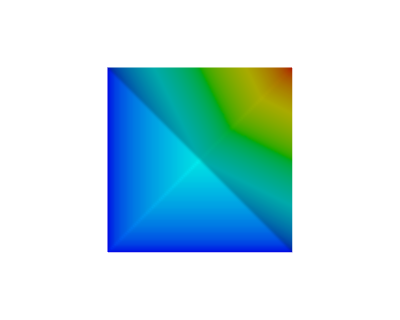
\includegraphics[width=0.3\textwidth]{pwld_3}}
\subfloat[Fourth basis function]{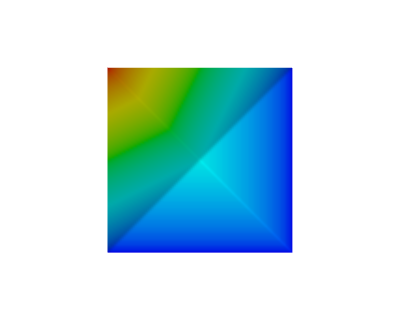
\includegraphics[width=0.3\textwidth]{pwld_4}}
\caption{PWLD basis function}
\label{pwld}
\end{figure}
On triangular cells, the PWLD basis functions reduces to the standard LD basis 
functions. Since the PWLD basis functions are built on triangular ``side'' 
sub-cells, the integrals over the area of a cell is replaced by a sum of integrals 
over the sides of the cell. 

After defining the spatial discretization that we employ here, we can now
define the Modified Interior Penalty DSA \cite{mip}. This DSA scheme uses 
discontinuous Galerkin finite elements for the spatial discretization and has
been shown to be always stable for isotropic scattering on triangular cells. 
The MIP weak form can be written as:
\begin{equation}
b(\phi,\phi^*) = l(\phi^*)
\label{mip}
\end{equation}
with:
\begin{equation}
\begin{split}
b(\phi,\phi^*) =& \(\Sigma_a \phi,\phi^*\)_{\mc{D}}+
(\mathrm{D}\bn\phi,\bn\phi^*)_{\mc{D}} + \(\kappa_e \llb\phi\rrb,
\llb\phi^*\rrb\)_{E_h^i} + \(\llb\phi\rrb,\ldb\mathrm{D}\partial_n
\phi^*\rdb\)_{E_h^i} +\\
& \(\ldb\mathrm{D}\partial_n \phi\rdb,\llb\phi^*\rrb\)_{E_h^i} + \(\kappa_e
\phi,\phi^*\)_{\partial \mc{D}^d} -\frac{1}{2} \(\phi,\mathrm{D} \partial_n
\phi^*\)_{\partial \mc{D}^d} - \frac{1}{2}\(\mathrm{D}\partial_n
\phi,\phi^*\)_{\partial \mc{D}^d}
\label{mip_b}
\end{split}
\end{equation}
\begin{equation}
l(\phi^*) = (Q_0,\phi^*)_{\mc{D}}+ (J^{inc},\phi^*)_{\partial \mc{D}^r}
\label{mip_l}
\end{equation}
where $(f,g)_{\mc{D}} = \sum_{K\in \mathbb{T}_h} \(f,g\)_K$, 
$(f,g)_K = \int_K fg\ d\br$, $(f,g)_{E_h^i}=\sum_{e\in E_h^i}(f,g)_e$, 
$(f,g)_e = \int_e fg\ ds$, $Q_0 = \Sigma_{s,0} \delta \phi^{(l)}$, 
$J^{inc} = \sum_{\bo\cdot\bs{n}_b >0} w_m |\bo_m \cdot \bs{n}_b| \delta
\psi_m^{(l)}$, $\mathbb{T}_h$ is the mesh used to discretize the domain
$\mc{D}$ into nonoverlapping elements $K$, $E_h^i$ is the set of interior
edges, $\mc{D}$  is the spatial domain, $\partial \mc{D}^d$ is the boundary of
the domain with Dirichlet condition, $\partial \mc{D}^r$ is the boundary of
the domain with reflective condition, $\Sigma_a$ is the absorption macroscopic
cross section, D is the diffusion coefficient, $\bs{n}_b$ is the outward
normal unit vector, $\partial_n = \bs{n}_e\cdot \bn$ where $\bs{n}_e$ is the 
normal unit vector associated with a given edge $e$, 
$\llb\phi\rrb = \phi^+ - \phi^-$ is the jump of $\phi$ at the interface between 
two elements, $\ldb\phi\rdb = \frac{\phi^+ + \phi^-}{2}$ is the mean of $\phi$ 
at the interface between two elements, 
$\phi^{\pm}=\lim_{s\rightarrow^{\pm}}\phi(\bs{r}+s\bs{n}_e)$, and
$\kappa_e = \max\(\kappa_e^{IP},\frac{1}{4}\)$
with:
\begin{equation}
\kappa_e^{IP} = \left\{
\begin{aligned}
&\frac{c(p^+)}{2} \frac{\mathrm{D^+}}{h_{\bot}^+} + \frac{c(p^-)}{2}
\frac{\mathrm{D}^-}{h_{\bot}^-} & \textrm{on interior edges, i.e., }
e\in E_h^i\\
&c(p) \frac{\mathrm{D}}{h_{\bot}} & \textrm{on boundary edges, i.e., } e
\in\partial \mc{D}^d 
\end{aligned}
\right. 
\end{equation}
where $c(p)$ is given by $c(p) = 2p (p+1)$, $p$ is the polynomial order ($p=1$
in this paper) and $h_{\bot}$ is the length of the cell in the direction
orthogonal to the edge $e$. On triangular cells, $h_{\bot}=\frac{2A}{L_e}$
with $A$ the area of the triangle and $L_e$ the length of the edge $e$. This
form of MIP was developed for discontinuous finite elements on triangular
cells. Once $\epsilon^{(l+1/2)}=\phi$ is obtained by solving \cref{mip}, the 
scalar flux and, when there is reflective boundaries, the angular fluxes can 
be corrected using:
\begin{align}
\Psi_m^{(l+1)} &= \Psi_m^{(l+1/2)} + \epsilon_m^{(l+1/2)}\\
\Phi^{(l+1)} &= \Phi^{(l+1/2)} + \varepsilon^{(l+1/2)}
\end{align}
By assuming that the angular dependence satisfies a diffusion expansion, the
angular correction can be computed as soon as the scalar flux correction is
known:
\begin{equation}
\epsilon_m^{(l+1/2)} = \frac{1}{4\pi} \(\varepsilon^{(l+1/2)} - 3D \bo_m\cdot \bn 
\varepsilon^{(l+1/2)}\)
\end{equation}

If PWLD finite elements are used, \cref{mip_b,mip_l} become:
\begin{equation}
\begin{split}
b(\phi,\phi^*) =& \la\Sigma_a \phi,\phi^*\ra_{\mc{D}}+
\la\mathrm{D}\bn\phi,\bn\phi^*\ra_{\mc{D}} + \(\kappa_e \llb\phi\rrb,
\llb\phi^*\rrb\)_{E_h^i} + \(\llb\phi\rrb,\ldb\mathrm{D} 
\partial_n\phi^*\rdb\)_{E_h^i} +\\
& \(\ldb\mathrm{D}\partial_n \phi\rdb,\llb\phi^*\rrb\)_{E_h^i} + \(\kappa_e
\phi,\phi^*\)_{\partial \mc{D}^d} -\frac{1}{2} \(\phi,\mathrm{D} \partial_n
\phi^*\)_{\partial \mc{D}^d} - \frac{1}{2}\(\mathrm{D}\partial_n
\phi,\phi^*\)_{\partial \mc{D}^d}
\label{mip_b_pwld}
\end{split}
\end{equation}
\begin{equation}
l(\phi^*) = \la Q_0,\phi^*\ra_{\mc{D}}+ \(J^{inc},\phi^*\)_{\partial \mc{D}^r}
\label{mip_l_pwld}
\end{equation}
where $\la f,g\ra_{\mc{D}} = \sum_{K\in \mathbb{T}_h} \la f,g\ra_{K}$, 
$\la f,g \ra_K = \sum_{s=1}^{V_K} \int_{K_s} fg\ d\br$, $K_s$ is a ``side'' 
sub-cell and $V_K$ is the number of vertices of cell $K$.
When the cells are not triangular, there is no simple way to know
$h_{\bot}$. To simplify the calculation of $h_{\bot}$, we assume that the
polygonal cells are not too far from being regular polygonal cells. If the
cell has an even number of edges, we assume that the orthogonal length is two
times the apothem
$\(\textrm{apothem}=2\times\frac{\textrm{area}}{\textrm{perimeter}}\)$. If the 
cell has an odd number of edges, we assume that the length is the apothem plus the 
circumradius $\(\textrm{circumradius}=\sqrt{\frac{2\times \textrm{area}}{V
\sin\(\frac{2\pi}{V}\)}}\)$. Therefore, $h_{\bot}$ is given by:
\begin{table}[H]
\begin{center}
\begin{tabular}{|c|c|c|c|c|}
\hline
Number of edges & 3 & 4 & $\geq 3$ and odd number & $\geq 4$ and even number\\
\hline
$h_{\bot}$ & $2 \times \frac{\textrm{area}}{L_e}$ &
$\frac{\textrm{area}}{L_e}$ & $4\times
\frac{\textrm{area}}{\textrm{perimeter}}$ & $2 \times
\frac{\textrm{area}}{\textrm{perimeter}}+\sqrt{\frac{2\times
\textrm{area}}{V\sin\(\frac{2\pi}{V}\)}}$\\
\hline
\end{tabular}
\caption{$h_{\bot}$ for different cells.}
\end{center}
\end{table}
